\documentclass[10pt]{article}

%----------------------------------------------------------------------------------------
%	Packages and configuration
%----------------------------------------------------------------------------------------

\usepackage[T1]{fontenc}
\usepackage{ucs} % Encoding errors
\usepackage[francais]{babel}
\usepackage{xltxtra} % More XELATEX
\usepackage{graphicx} % Permits to include some pictures
\usepackage{fontspec}
\usepackage{url} % Url links
\usepackage{float} % Adds options to floats like H
\usepackage[ocgcolorlinks]{hyperref}
\usepackage{fancyhdr}
\usepackage{metalogo}
\usepackage[titletoc]{appendix}
\usepackage{pdflscape} % Pour des pages au format paysage
\usepackage{enumitem}  % Pour pouvoir choisir le symbole de itemize : 
                       % \begin{itemize}[label={$\bullet$}]
\usepackage{tabu}
\usepackage{tabularx}
\usepackage{multirow}
\usepackage{lastpage}
\usepackage{multicol}
\usepackage{wrapfig}
\usepackage{longtable}
\usepackage[left=3.5cm,right=3.5cm,top=2cm,bottom=2cm]{geometry} % Change margins
\usepackage[square]{natbib}
\hypersetup{colorlinks=true,allcolors=black}

\setmainfont{Sorts Mill Goudy}
% \setmainfont[BoldFont={Exo},
%   BoldFeatures={Weight=4,Scale=0.9}]{Sorts Mill Goudy}

% \usepackage{sectsty}
% \allsectionsfont{
%   \fontspec[BoldFont={Sorts Mill Goudy}]{Sorts Mill Goudy}}
\pagenumbering{arabic}
\urlstyle{same}
\tabulinesep =1mm
%----------------------------------------------------------------------------------------
%	Header
%----------------------------------------------------------------------------------------

\newcommand{\helv}{%
   \fontsize{9}{11}\selectfont}

   \lhead{\helv \parbox[b]{3.0cm}{ÉTS - Département de génie logiciel et des TI}}
   \chead{\helv \parbox[b]{7cm}{\centering LOG792 - Rapport d'étape - Optimisation des paramètres d’une éolienne en mouvement}}
\rhead{\helv \today \linebreak \thepage}
\lfoot{}
\cfoot{}
\rfoot{}

\setlength{\headwidth}{\textwidth}
\setlength{\headheight}{23pt}

\renewcommand{\headrulewidth}{0.4pt}
%\renewcommand{\footrulewidth}{0.4pt}

%----------------------------------------------------------------------------------------
%	Document
%----------------------------------------------------------------------------------------

\begin{document}

\pagestyle{fancy}

%----------------------------------------------------------------------------------------
%	Page titre
\begin{titlepage}
\thispagestyle{fancy}

\newcommand{\HRule}{\rule{\linewidth}{0.5mm}} % Defines a new command for the horizontal lines, change thickness here

\center % Center everything on the page
 
%----------------------------------------------------------------------------------------
%	HEADING SECTIONS
%----------------------------------------------------------------------------------------

\textsc{\LARGE École de Technologie Supérieure}\\[1.5cm] % Name of your university/college

\vfill

\textsc{\Large Rapport d'étape}\\[0.5cm] % Major heading such as course name
\textsc{\large Projet de fin d'études \\ Département de génie logiciel et des TI}\\[0.5cm] % Minor heading such as course title

%----------------------------------------------------------------------------------------
%	TITLE SECTION


\HRule \\[0.4cm]
{ \huge \bfseries Optimisation des paramètres d’une éolienne en mouvement}\\[0.4cm] % Title of your document
\HRule \\[1.5cm]
 
%----------------------------------------------------------------------------------------
%	AUTHOR SECTION

\begin{minipage}{0.4\textwidth}
\begin{flushleft} \large
\emph{Auteur:}\\
Pierre-Alexandre \textsc{St-Jean}\\
\small{<pa@stjean.me>}
\end{flushleft}
\end{minipage}
~
\begin{minipage}{0.4\textwidth}
\begin{flushright} \large
\emph{Superviseur:} \\
Dr. Christian \textsc{Desrosiers}\\
\small{<christian.desrosiers@etsmtl.ca>}
\end{flushright}
\end{minipage}\\[4cm]

\vfill

%----------------------------------------------------------------------------------------
%	DATE SECTION


{\large \today}\\[3cm] % Date, change the \today to a set date if you want to be precise

%----------------------------------------------------------------------------------------
%	LOGO SECTION

%\includegraphics{Logo}\\[1cm] % Include a department/university logo - this will require the graphicx package

 

\end{titlepage}



%----------------------------------------------------------------------------------------
%	Table des matières
\section*{Table des matières}
% \addcontentsline{toc}{section}{Table des matières}
\renewcommand{\contentsname}{Table des matières}
\makeatletter
\renewcommand{\tableofcontents}{\@starttoc{toc}%
}
\makeatother
\tableofcontents
\phantomsection
%\listoffigures
%\addcontentsline{toc}{section}{Table des figures}
%\clearpage

% \vspace*{\fill}
% \begin{center}

\clearpage
%\begin{multicols}{2}
%----------------------------------------------------------------------------------------
%	Abstract
\section*{Résumé}
\addcontentsline{toc}{section}{Résumé}

Le club étudiant Chinook de l'ÉTS afin de continuer son succès en compétition améliore continuellement son véhicule éolien. Un système de contrôle pour l'éolienne tel que celui présent dans les éoliennes statiques doit être mis en place afin d'améliorer la performance du véhicule. Le contrôle de l'angle d'attaque et de la vitesse de rotation de l'éolienne est la façon la plus commune d'ajuster la puissance de sortie d'une éolienne. Afin d'arriver à optimiser le système, l’éolienne du véhicule est d’abord caractérisée expérimentalement puis un système de contrôle de l'angle d'attaque et du ratio de transmission par algorithme génétique est développé, analysé et testé théoriquement et expérimentalement. Le système de contrôle utilisé n'est pas un système conventionnel (PI,PID,etc.) auquel une seule entrée et une seule sortie est considérée, mais plutôt un système dans l'espace d'état dans lequel plusieurs entrées et plusieurs sorties sont considérées.

Résumé des résultats à venir ...


%----------------------------------------------------------------------------------------
%	Intro
\section{Introduction} % (fold)
\label{sec:Introduction}

\subsection{Problématique et contexte} % (fold)
\label{sub:prob_contexte}

Le club étudiant Chinook\footnote{\url{http://chinookets.com}} de l'ÉTS est un regroupement d'étudiants qui analysent, concoivent et construisent un véhicule propulsé par une éolienne [figure \ref{fig:chinookHall}]. Le véhicule participe, chaque année, depuis deux années à une compétition de véhicules du même type et participe à des courses contre la montre. Le véhicule est ensuite évalué selon sa performance en fonction de sa vitesse par rapport à la vitesse du vent.

La compétition vise à ammener les étudiants a développer de nouvelles technologies pour les éoliennes, plus précisément pour des éoliennes de petites dimensions. Afin de rendre la compétition intéressante, elle sont utilisées en tant que moteur d'un véhicule de petite dimension. Un tel véhicule ne serait pas viable mais une telle technologie pourrait facilement être adapté sur d'autre médiums tels que les éoliennes sur des navires ou pour des batiments.

\begin{figure}[H]
  \centering
  \includegraphics[width=0.5\textwidth]{images/chinook_1_2.jpg}
  \caption[Chinook 1 et 2]{Le Chinook 1 et le Chinook 2 en exposition dans le Hall A de l'ÉTS}
  \label{fig:chinookHall}
\end{figure}

Pour améliorer le véhicule, permettre de à l'équipe de bien performer et rester compétitif l'équipe installe un système électro-mécanique de contrôle de l'angle d'attaque des pâles. La transmission du véhicule sera aussi modifiée afin de pouvoir être asservi électroniquement.

Afin de pouvoir contrôller ces systèmes électroniques, des modèles de contrôle et d'optimisation de la puissance de l'éolienne doivent être créés. Les modèles disponibles sur les éoliennes statique peuvent s'appliquer pour une éolienne en mouvement mais doivent être modifiés afin de prendre en compte plusieurs facteurs.

\citet{LaksPao} décris plusieurs méthodes de contrôle des éoliennes mais la plupart de ces méthodes ne vont pas chercher le point maximum de puissance, elle vont plutôt chercher un point stable de contrôle qui permet d'offrir une puissance stable pour les générateurs électrique. \citet{Jelavic05} va chercher le point maximum de puissance de l'éolienne, mais seulement dans le cas oùla vitesse du vent est sous la vitesse prescrite de l'éolienne. \citet{Ouissam12} dans son article utilise un algorithme génétique couplé a un algorithme flou (fuzzy control system), la méthode semble fonctionner mais celui-ci ne semble pas prendre en compte les changements de vitesse de rotation de l'éolienne et les variations de la vitesse du vent.

% subsection Problématique et contexte (end)
\subsection{Objectifs} % (fold)
\label{sub:Objectifs}


Le présent projet à pour but d'ammener l'éolienne du Chinook 3 [figure: \ref{fig:matRotor}] à opérer dans les conditions et à l'aide des paramètres d'opérations les plus optimales possibles. Pour ce faire, l'éolienne doit être caractérisé, un modèle de contrôle et d'optimisation de l'angle d'attaque ($\beta$) des pales et du ratio de transmission qui affecte la vitesse de rotation de l'éolienne ($\omega$) doit être conçu, analysé puis ce modèle doit être implanté dans le logiciel de la carte électronique de calcul.

Le système de contrôle pourra, à tout moment et selon certaines conditions, changer l'angle d'attaque des pales ($\beta$) où le ratio transmission afin d'atteindre les performances optimales de l'éolienne dans les conditions de vitesse du véhicule et de vitesse du vent.

\begin{figure}[H]
  \centering
  \includegraphics[width=0.5\textwidth]{images/mat_rotor_annote.jpg}
  \caption[Mat et Rotor du Chinook 3]{Rendu 3D du mat et du rotor du Chinook 3}
  \label{fig:matRotor}
\end{figure}

Un tel modèle ainsi opérationnel dans les systèmes de contrôle du Chinook permettra au véhicule d'atteindre de meilleures vitesses et ce plus rapidement tout en permettant de conserver les vitesses atteintes et de mieux résister aux turbulences environnementales que par les années passées.

% subsection Objectifs du projet (end)

% section Introduction (end)


%----------------------------------------------------------------------------------------
%	Methodologie
\section{Méthodologie} % (fold)
\label{sec:Méthodologie}

La méthode de résolution du problème peut être résumée par étape : 

\begin{enumerate}
\item Caractérisation du $C_p$ (efficacité) de l 'éolienne
\item Modélisation de l'espace d'état
\item Modélisation de l'algorithme génétique
\item Modélisation du système de contrôle
\item Implémentation sur la carte de calcul
\end{enumerate}

\subsection{Analyse du modèle} % (fold)
\label{sub:Analyse du modèle}

La puissance de l'éolienne est donné par :
\begin{equation}
\label{eqn:peol}
P_t= \frac{1}{2} \rho \pi R^2 C_p(\lambda,\beta)v^3
\end{equation}

Où:

\begin{itemize}
\item $P_t$ : la puissance de sortie de l'éolienne (watts)
\item $\rho$ : la densité de l'air ambiante ($\approx 1.225kg/m^3$)
\item $R$ : le rayon de l'éolienne (m)
\item $\lambda$ : le ratio de vitesse en bout de pale (tip-speed ratio)
                  \begin{equation}
                  \lambda = \frac{\omega_t * R}{v}
                  \end{equation}
\item $\omega_t$ : la vitesse de rotation de l'éolienne (rad/s)
\item $\beta$ : l'angle d'attaque des pales (rad)
\item $C_p$ : l'efficacité de l'éolienne en fonction de l'angle d'attaque des pales et du ratio n de vitesse en bout de pale
\item $v$ : la vitesse de vent relative à l'éolienne (m/s)
\end{itemize}

Le coefficient de puissance de l'éolienne peut être obtenu à l'aide de cette équation:

\begin{equation}
C_p(\lambda,\beta) = c_1 (\frac{c_2}{\lambda_i}-c_3*\beta - c_4) e^{-\frac{c_5}{\lambda_i}} + c_6 \lambda
\end{equation}

Où:

\begin{equation}
\frac{1}{\lambda_i} = \frac{}{} + \frac{0.035\lambda+0.08\beta}{1+\beta^3} 
\end{equation}


Le torque produit de l'éolienne est défini comme:

\begin{equation}
T_t = \frac{P_t}{\omega_t}
\end{equation}

\subsubsection{Caractérisation du $C_p$ (efficacité) de l 'éolienne}

La caractérisation de l'éolienne est effectuée expérimentalement. On récupère les données de torque, de vitesse de rotation, de vitesse de vent et d'angle d'attaque et on fais une régression paramétrique sur l'équation $C_p$ afin de trouver tout les constantes $c_1 ... c_6$.

Premièrement on doit isoler$C_p$ dans l'équation mécanique de puissance à l'aide de l'accélération angulaire:

\begin{equation}
  \label{eqn:paccel}
  P= I \alpha
\end{equation}

Avec $I$ l'inertie totale du système qui pour la plateforme de test du Chinook est de $0.788195$
et $\alpha$ qui est l'accélération angulaire ($rad/s^2$) de l'éolienne.

À l'aide de l'équation \ref{eqn:peol} et \ref{eqn:paccel} on peut faire une régression paramétrique de type Levenberg-Marquardt afin de trouver les paramètres  $c_1 ... c_6$.

\subsubsection{Modélisation de l'espace d'état}

La modélisation dans l'espace d'état \citep{wiki_statespace} est un modèle mathématique du système complet de l'éolienne et du Chinook. Une telle représentation permet de connaître l'état de ce système selon les variables d'entrée les variables de sorties et les états.

L'état du système peut être représenté par ces équations:

\begin{equation}
\dot{\mathbf{x}}(t) = A(t) \mathbf{x}(t) + B(t) \mathbf{u}(t)
\end{equation}
\begin{equation}
\mathbf{y}(t) = C(t) \mathbf{x}(t) + D(t) \mathbf{u}(t)
\end{equation}

\begin{itemize}
  \item $\mathbf{x}(\cdot)$ est le vecteur d'état
  \item $\mathbf{y}(\cdot)$ est le vecteur de sortie
  \item $\mathbf{u}(\cdot)$ est le vecteur de contrôle
  \item $A(\cdot)$ est la matrice d'état
  \item $B(\cdot)$ est la matrice de contrôle
  \item $C(\cdot)$ est la matrice de sortie
  \item $D(\cdot)$ est la d'action directe
\end{itemize}

L'espace d'état peut aussi être représenté par le graphique à la figure \ref{fig:statespace}.

\begin{figure}[H]
\label{fig:statespace}
\centering
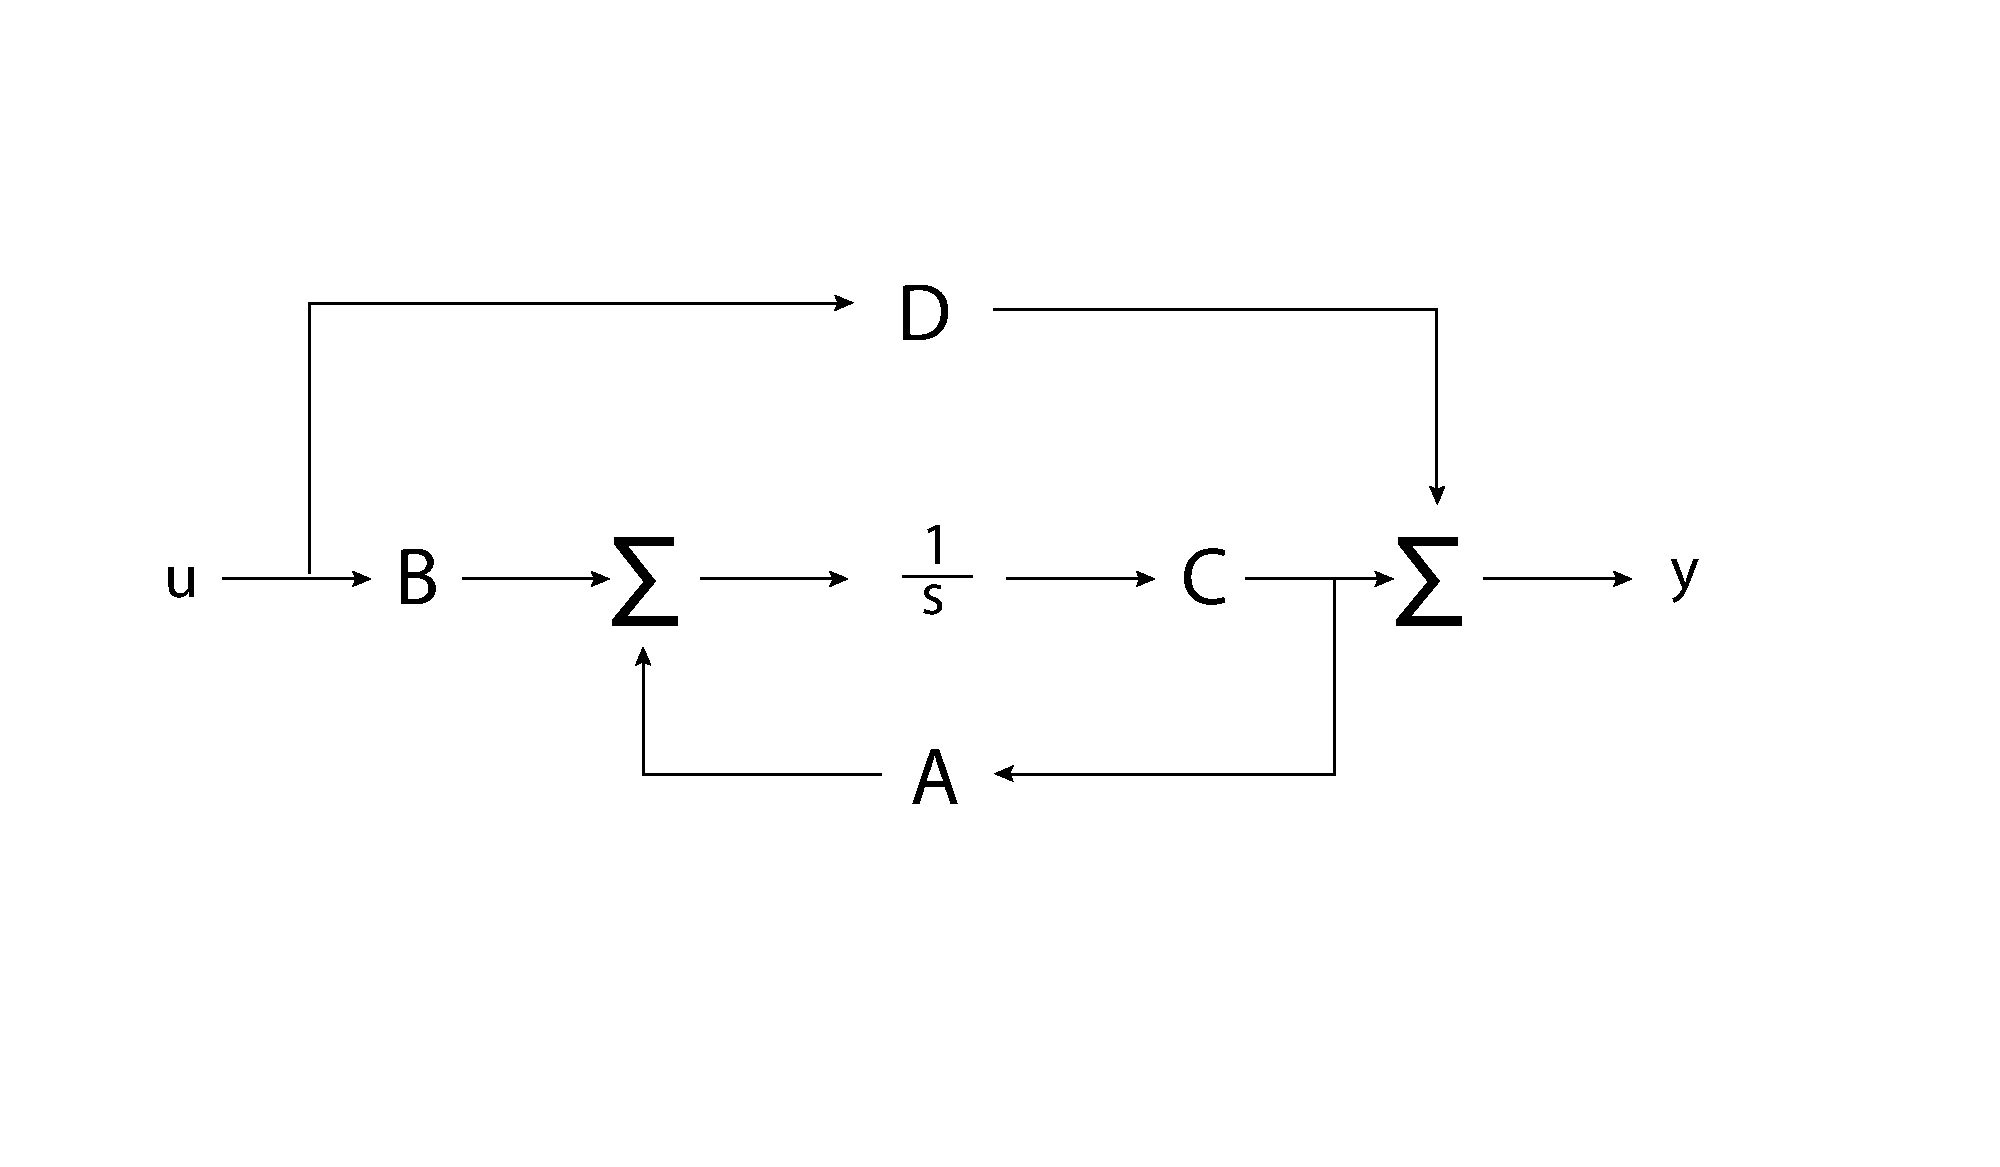
\includegraphics[width=0.8\textwidth]{images/statespace.pdf}
\caption{Représentation en bloque de l'espace d'état}
\end{figure}


... La modélisation des équations dans l'espace d'état suivra.

\subsubsection{Modélisation de l'algorithme génétique}

La méthodologie pour la modélisation de l'algorighme génétique de maximisation de la puissance de l'éolienne n'est pas encore fait et viendra.

\subsubsection{Modélisation du système de contrôle}

La méthodologie pour la modélisation du système de contrôle de l'éolienne n'est pas encore fait et viendra.

% subsection Analyse du modèle (end)
\subsection{Intégration du modèle} % (fold)
\label{sub:Intégration du modèle}

Le modèle après analyse doit être intégré à l'intérieur de la carte électronique de calcul (figure \ref{fig:carte}) conçu à cette fin. C'est une carte composée d'un microcontrôlleur 16 bit de 70 mips ayant 512 KB d'espace programme et 50 KB de mémoire vive

\begin{figure}[H]
\label{fig:carte}
\centering
\begin{tabular}{cc}
\includegraphics[width=0.4\textwidth]{images/carte-electronique-dessus.jpg} &
\includegraphics[width=0.4\textwidth]{images/carte-electronique-dessous.jpg}
\end{tabular}
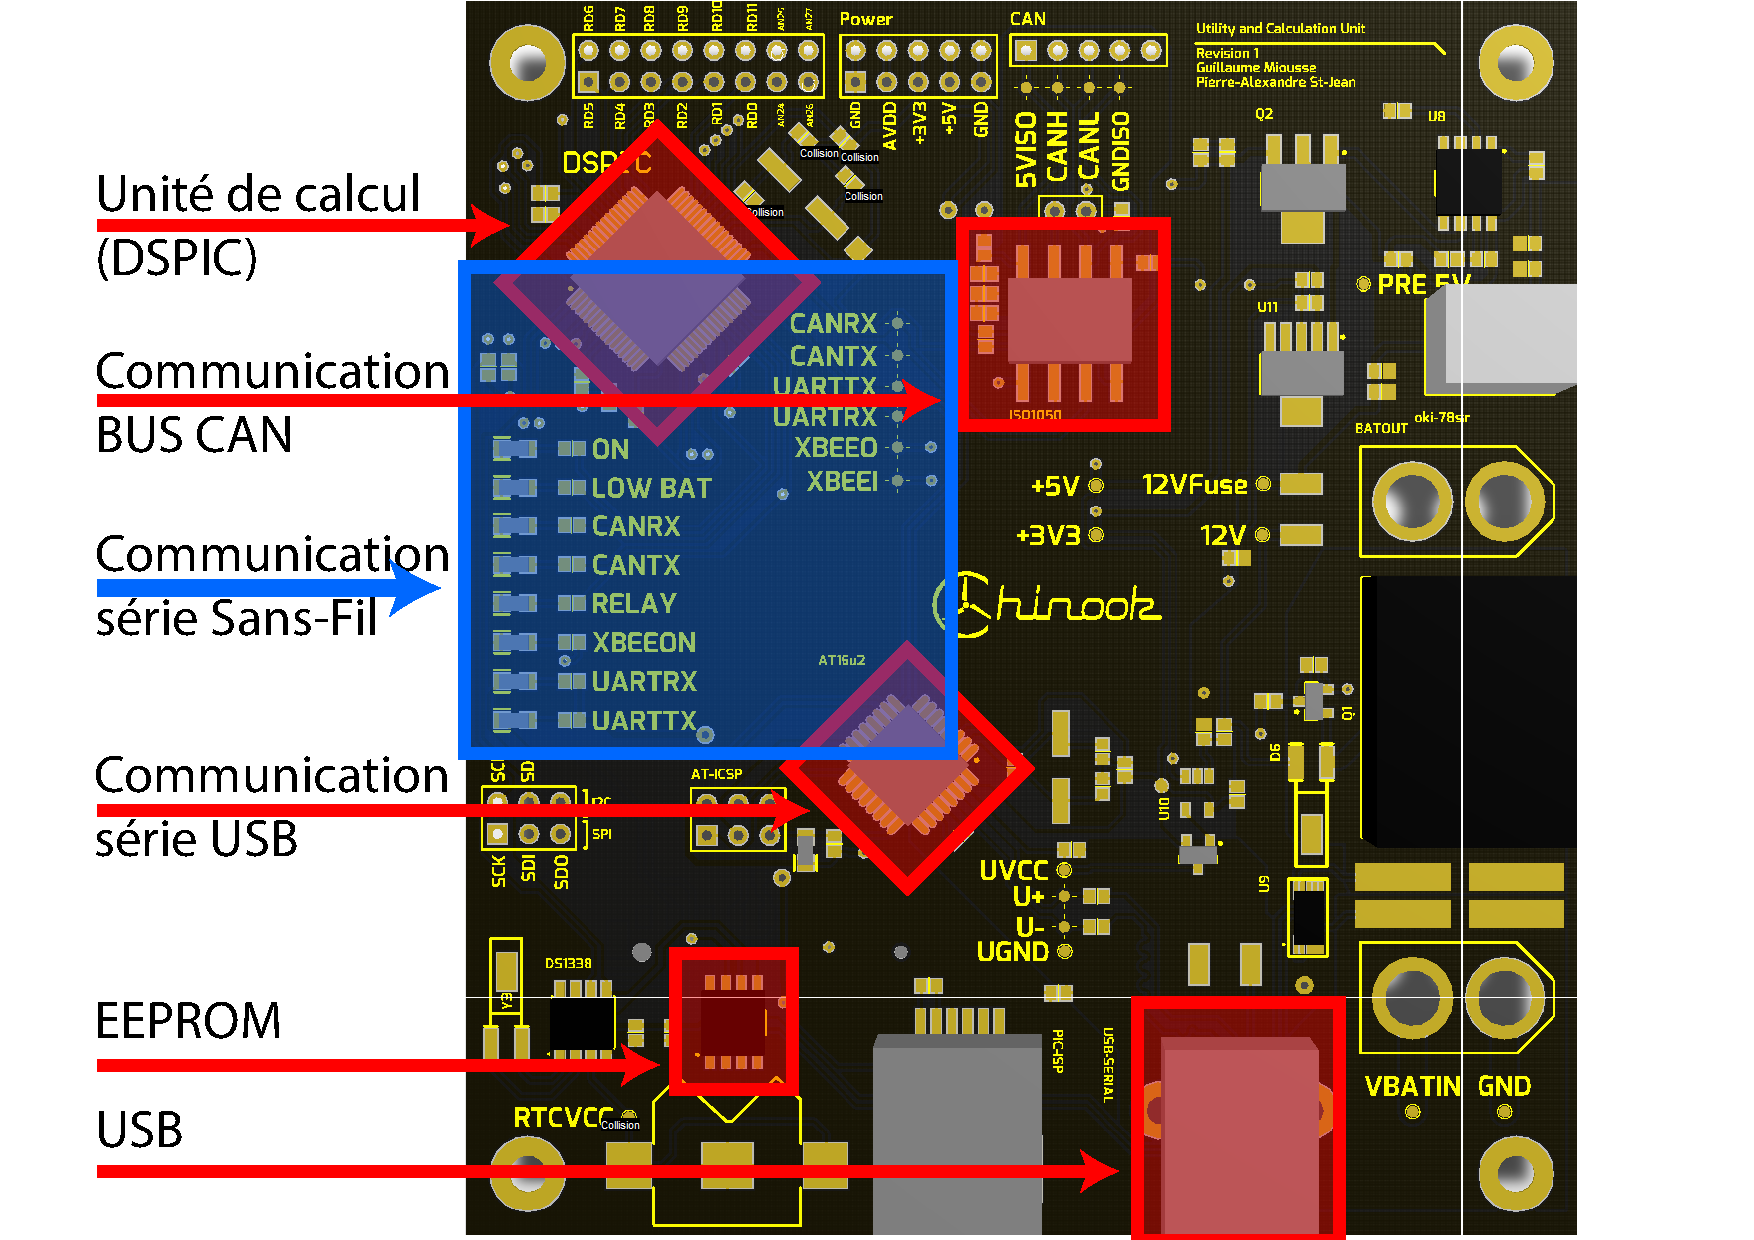
\includegraphics[width=0.6\textwidth]{images/carte-electronique-annote.pdf}
\caption{La carte électronique de calcul}
\end{figure}

Le code de contrôle doit y être intégré. Premièrement les bibliothèques de communication et l'application qui petmet de faire fonctionner la carte doit fonctionner. Puis on intègre le modèle mathématique en le transformant en programme en C utilisant les données reçus des autres cartes.

% subsection Intégration du modèle (end)
\subsection{Gestion du projet} % (fold)
\label{sub:Gestion du projet}



% subsection Gestion du projet (end)
% section Méthodologie (end)


%----------------------------------------------------------------------------------------
%	Resultats
\section{Résultats} % (fold)
\label{sec:resultats}

\subsection{Sommaire des travaux réalisés} % (fold)
\label{sub:Sommaire des travaux réalisés}

% subsection Sommaire des travaux réalisés (end)
\subsection{Recommandations} % (fold)
\label{subsec:Recommandations}

% subsection Recommandations (end)
% section resultats (end)


%\end{multicols}
%----------------------------------------------------------------------------------------
%	Resultats
\section{Planification} % (fold)
\label{sec:Planification}

% TODO: Mettre la planification ici0

\subsection{Artéfacts} % (fold)
\label{sub:artefacts}

% subsection Description des artéfacts (end)
\subsection{Risques} % (fold)
\label{sub:Risques}

% subsection Risques (end)
% section Planification (end)


\bibliographystyle{annotate}
%\bibliographystyle{apalike}
%\bibliographystyle{plainnat}
%\bibliographystyle{development}
\bibliography{bibliography}
\addcontentsline{toc}{section}{Références}

%\clearpage

%----------------------------------------------------------------------------------------
%	Annexes
%----------------------------------------------------------------------------------------
\section*{Annexes}
\addcontentsline{toc}{section}{Annexes}
\begin{appendices}



\end{appendices}

\end{document}


